%%%%%%%%%%%%%%%%%%%%%%%%%%%%%%%%%%%%%%%%%
% Beamer Presentation
% LaTeX Template
% Version 1.0 (10/11/12)
%
% This template has been downloaded from:
% http://www.LaTeXTemplates.com
%
% License:
% CC BY-NC-SA 3.0 (http://creativecommons.org/licenses/by-nc-sa/3.0/)
%
%%%%%%%%%%%%%%%%%%%%%%%%%%%%%%%%%%%%%%%%%

%----------------------------------------------------------------------------------------
%	PACKAGES AND THEMES
%----------------------------------------------------------------------------------------

\documentclass{beamer}

\mode<presentation> {
\usetheme{Warsaw}
\usetheme{metropolis}  
%\setbeamertemplate{footline} % To remove the footer line in all slides uncomment this line
%\setbeamertemplate{footline}[page number] % To replace the footer line in all slides with a simple slide count uncomment this line

%\setbeamertemplate{navigation symbols}{} % To remove the navigation symbols from the bottom of all slides uncomment this line
}
%\setbeamertemplate{background}
%{\includegraphics[width=\paperwidth,height=\paperheight,keepaspectratio]{background.jpg}}
\usepackage{graphicx} % Allows including images
\usepackage{booktabs} % Allows the use of \toprule, \midrule and \bottomrule in tables

%----------------------------------------------------------------------------------------
%	TITLE PAGE
%----------------------------------------------------------------------------------------

\title[GECO ]{STREAM 3D project} % The short title appears at the bottom of every slide, the full title is only on the title page

\author{D. Cerroni, L. Formaggia, A. Scotti and P. Zunino} % Your name
\institute[MOX laboratory, Department of Mathematics] 
{
Politecnico di Milano\\ % Your institution for the title page
\medskip
%\textit{daniele.cerroni} % Your email address
}
\date{\today} % Date, can be changed to a custom date
\usepackage{tikz}
\usepackage{amsmath}
\usepackage{verbatim}
\usetikzlibrary{arrows,shapes}
\renewcommand\mathfamilydefault{\rmdefault}



\setbeamertemplate{background}
{
\includegraphics[width=\paperwidth,height=\paperheight]{figure/back}}

\begin{document}

\begin{frame}
\titlepage % Print the title page as the first slide
\end{frame}
%%%%%%%%%%%%%%%%%%%%%%%%%%%%%%%%%%%%%%%%%%%%%
\begin{frame}
\frametitle{Overview} % Table of contents slide, comment this block out to remove it
\tableofcontents % Throughout your presentation, if you choose to use \section{} and \subsection{} commands, these will automatically be printed on this slide as an overview of your presentation
\end{frame}
%%%%%%%%%%%%%%%%%%%%%%%%%%%%%%%%%%%%%%%%%%%%%%%
\section{Introduction}
%%%%%%%%%%%%%%%%%%%%%%%%%%%%%%%%%%%%%%%%%%%%%%%
\begin{frame}{Background and Motivations}
\begin{columns}
\begin{column}{0.65\textwidth}
\begin{block}{Key processes of sedimentary basin evolution:} 
\begin {itemize}
\item  geomechanics and dynamic evolution of stress and deformations; 
\item  transport of dissolved chemicals; 
\item geochemical reactive processes.
\end{itemize}
\end{block}
\begin{block}{The effects of glaciations on the subsurface:} 
\begin {itemize}
\item  the mechanical compaction due to the load of ice sheets; 
\item  the deformation of the lithosphere by isostasy; 
\item  the subglacial meltwater; 
\item  the generation of permafrost. 
\end{itemize}
\end{block}
\end{column}
\begin{column}{0.35\textwidth}
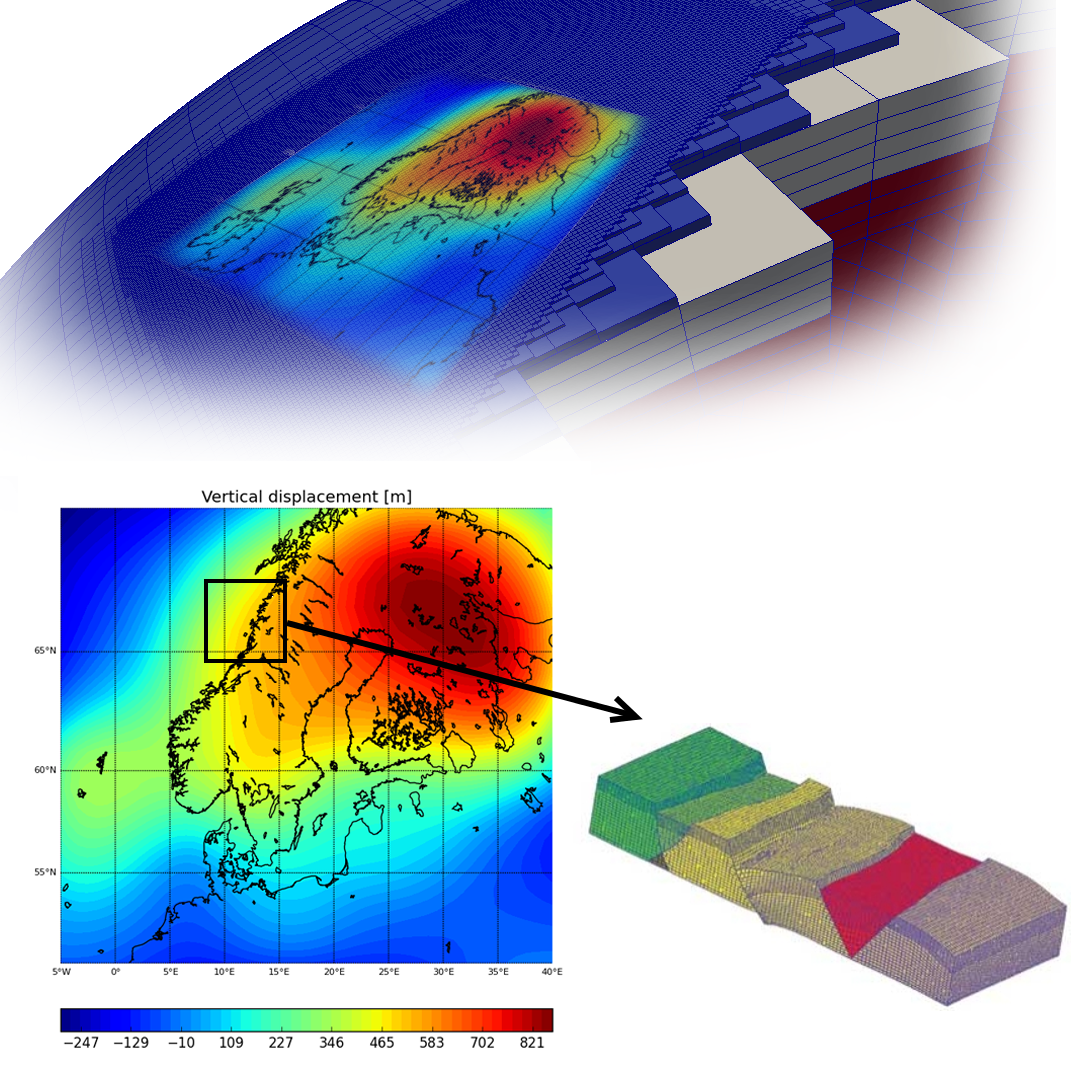
\includegraphics[width=0.9\textwidth]{figure/intro1}
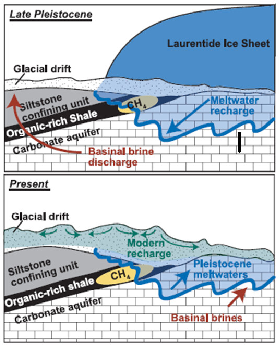
\includegraphics[width=0.9\textwidth]{figure/intro2}
\end{column}
\end{columns}
\end{frame}
%%%%%%%%%%%%%%%%%%%%%%%%%%%%%%%%%%%%%%%%%%%%%%%
\section{Mathematical model}
%%%%%%%%%%%%%%%%%%%%%%%%%%%%%%%%%%%%%%%%%%%%%%%
%%%%%%%%%%%%%%%%%%%%%%%%%%%%%%%%%%%%%%%%%
\begin{frame}{Poromechanics}
	\begin{align*}
 	-\nabla \cdot \left(  2\mu\varepsilon (\mathbf{u}) + \nabla\cdot \mathbf{u}\right) + \alpha \nabla p=\rho\mathbf{g} \, ,\\
 	\partial_t \left(\frac{p}{M} + \alpha \nabla \cdot \mathbf{u}\right)+ \nabla\cdot \mathbf{u_d}=S_f\,,\\ 
 	\mathbf{K}^{-1}\mathbf{u_d} + \nabla p = \rho_f\mathbf{g}\,,
 \end{align*}
\end{frame}
%%%%%%%%%%%%%%%%%%%%%%%%%%%%%%%%%%%%%%%%%%%%%%%%%
%%%%%%%%%%%%%%%%%%%%%%%%%%%%%%%%%%%%%%%%%
\begin{frame}{Temperature Dynamics}
	\begin{align*}
 	C_T\frac{\partial T}{\partial t} +
 	\left(  \phi\rho_l c_l \mathbf{v_l} 
 	+  (1 - \phi)\rho_s c_s \mathbf{v_s} \right)\cdot \nabla T- K_T \nabla^2 T 
 	= Q\,.
 \end{align*}
\end{frame}
%%%%%%%%%%%%%%%%%%%%%%%%%%%%%%%%%%%%%%%%%%%%%%%%%
%%%%%%%%%%%%%%%%%%%%%%%%%%%%%%%%%%%%%%%%%
\begin{frame}{Chemical transport}
	\begin{align*}
 	C_T\frac{\partial C}{\partial t} +
 	\mathbf{u_D} \cdot \nabla C- D\nabla^2 T 
 	= Q_c\,.
 \end{align*}
\end{frame}
%%%%%%%%%%%%%%%%%%%%%%%%%%%%%%%%%%%%%%%%%%%%%%%%%
%%%%%%%%%%%%%%%%%%%%%%%%%%%%%%%%%%%%%%%%%
\begin{frame}{Coupled model}
Poromechanics - Temperature Dynamics - Chemical transport
	\begin{align*}
 	-\nabla \cdot \left(  2\mu\varepsilon (\mathbf{u}) + \nabla\cdot \mathbf{u}\right) + \alpha \nabla p=\rho\mathbf{g} \, ,\\
 	\partial_t \left(\frac{p}{M} + \alpha \nabla \cdot \mathbf{u}\right)+ \nabla\cdot \mathbf{u_d}=S_f\,,\\ 
 	\mathbf{K}^{-1}\mathbf{u_d} + \nabla p = \rho_f\mathbf{g}\,,\\
 	C_T\frac{\partial T}{\partial t} +
 	\left(  \phi\rho_l c_l \mathbf{v_l} 
 	+  (1 - \phi)\rho_s c_s \mathbf{v_s} \right)\cdot \nabla T- K_T \nabla^2 T 
 	= Q\,.\\
 	C_T\frac{\partial C}{\partial t} +
 	\mathbf{u_D} \cdot \nabla C- D\nabla^2 T 
 	= Q_c\,.
 \end{align*}
\end{frame}
%%%%%%%%%%%%%%%%%%%%%%%%%%%%%%%%%%%%%%%%%%%%%%%%%
%%%%%%%%%%%%%%%%%%%%%%%%%%%%%%%%%%%%%%%%%%%%%%%
\section{Numerical Plattofrm}
%%%%%%%%%%%%%%%%%%%%%%%%%%%%%%%%%%%%%%%%%%%%%%%
%%%%%%%%%%%%%%%%%%%%%%%%%%%%%%%%%%%%
\begin{frame}{Numerical platform}
\begin{columns}
\begin{column}{0.45\textwidth}

\includegraphics[width=0.8\columnwidth]{figure/logogetfem}
\begin{block}{GetFem}
\begin{itemize}
\item c++ finite element platform
\item Generic assembly language
\item Level-set and finite element cut 
	by one or several level-set (Xfem) 
\end{itemize}
\end{block}
\end{column}
\begin{column}{0.45\textwidth}
\begin{block}{SAMG library}
Algebraic Multigrid Methods for Systems
\begin{itemize}
\item solution of large linear systems
\item higly scalable
\item easy to integrate
\end{itemize}
\end{block}
\end{column}
\end{columns}
\end{frame}
%%%%%%%%%%%%%%%%%%%%%%%%%%%%%%%%%%%%%%%%%%%%%
%%%%%%%%%%%%%%%%%%%%%%%%%%%%%%%%%%%%%
\begin{frame}{Geometric VS Algebraic}
\centering
\vfill
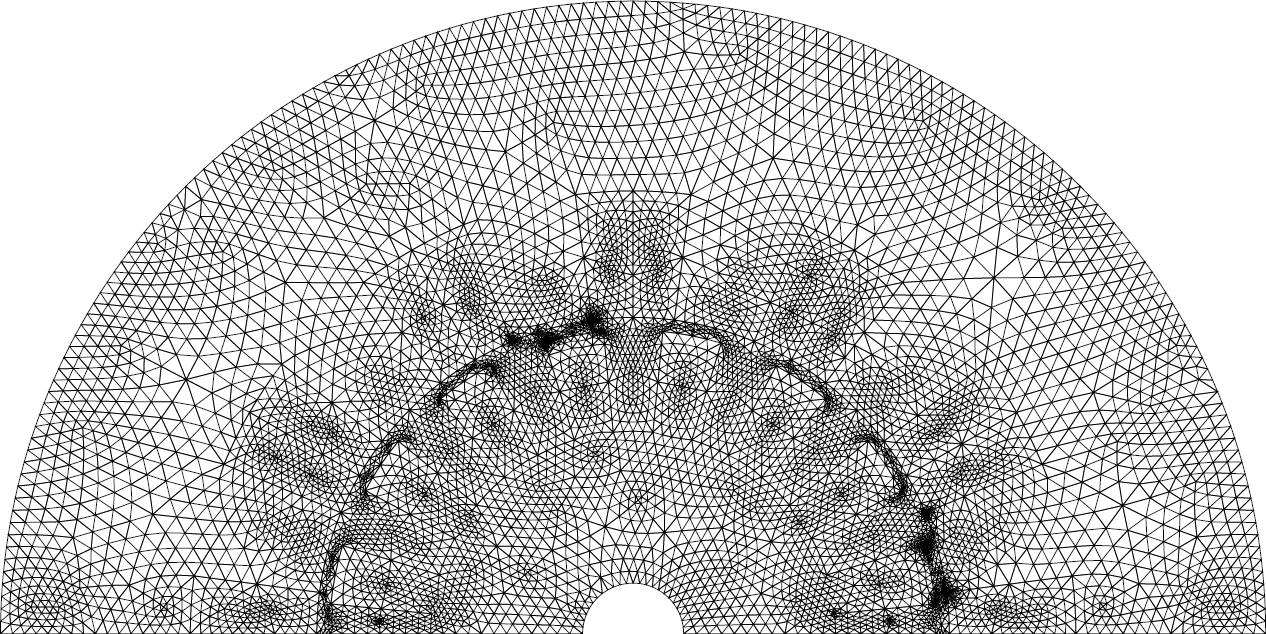
\includegraphics[width=0.7\textwidth]{figure/compex1.png}
\vfill
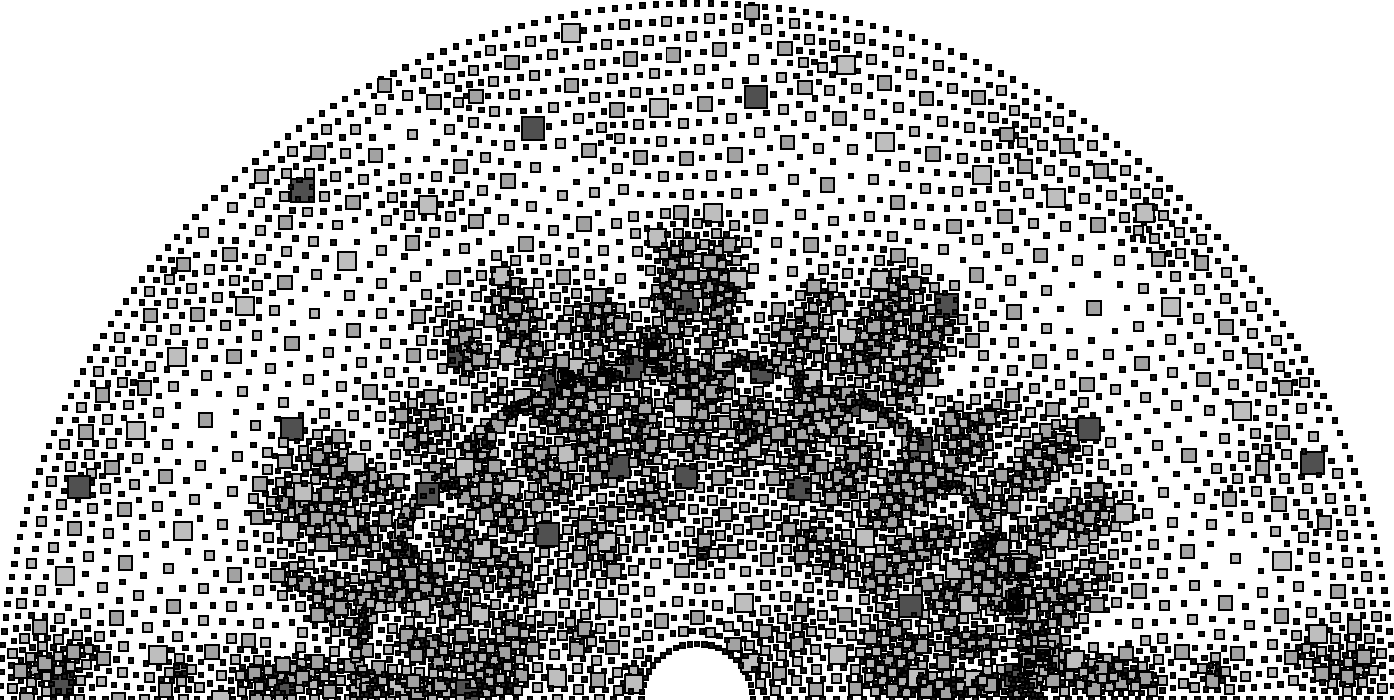
\includegraphics[width=0.7\textwidth]{figure/compex2.png}
\vfill
\end{frame}
%%%%%%%%%%%%%%%%%%%%%%%%%%%%%%%%%%%%%%
%%%%%%%%%%%%%%%%%%%%%%%%%%%%%%%%%%%%%%%%%%%%%
\begin{frame}{Integration}
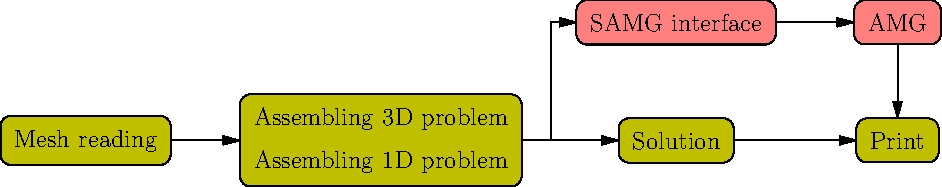
\includegraphics[width=0.9\textwidth]{figure/flowchart}
\begin{itemize}
\item Simple interface (CSR matrix)
\item Same programming language
\end{itemize}
\end{frame}
%%%%%%%%%%%%%%%%%%%%%%%%%%%%%%%%%%%%%%%%%%%%%%%%%%%%%%
%%%%%%%%%%%%%%%%%%%%%%%%%%%%%%%%%%%%%%%%%%%%%%%
\section{Conclusion}
%%%%%%%%%%%%%%%%%%%%%%%%%%%%%%%%%%%%%%%%%%%%%%%








\end{document}
